\section{Обзор литературы}
\label{sec:lit_review}

\subsection{Обзор существующих аналогов}
\label{sub:lit_review:analogues}
Разработанная в ходе дипломного проектировании система функционального контроля технических средств не имеет широко
известных прямых аналогов. Отсутствие конкурирующих систем вызвано тем следующими причинами:
\begin{itemize}
	\item технические средства, предназначенные для нужд армии имеют ограниченное распространение
	\item протоколы обмена данными между техническими средствами и ЭВМ зачастую являются закрытыми
	\item модуль функционального контроля зачастую является частью закрытого проприетарного ПО, используемого для
		автоматизации задач личного состава
	\item разнообразие устройств, протоколов обмена
\end{itemize}

Таким образом, ввиду невозможности поиска аналогов среди ПО для вооруженных сил, в данном разделе будут проанализированы
наиболее близкие аналоги из других областей.

Наиболее приближенным аналогом является система функционального применяемая на железных дорогах Российской федерации
~\cite{rus_rails}.

\begin{figure}[ht]
	\centering
	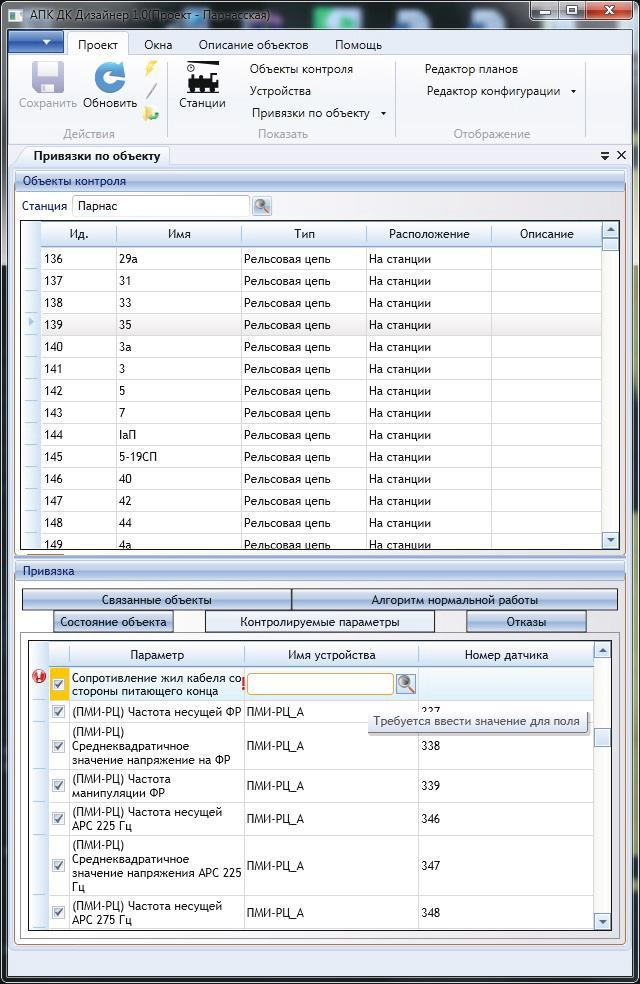
\includegraphics[scale=0.36]{rw_control}
	\caption{Модуль функционального контроля системы автоматизации РЖД~\cite{rus_rails}}
	\label{fig:lit_reiview:analogues:rw_control}
\end{figure}

Данная система функционального контроля позволяет проводить мониторинг различных участков железной дороги, оказывать
управляющие воздействия на объекты контроля, выводить информацию на экран или бумажный носитель, экспортировать данные в
другие программы для работы с результатами мониторинга.

Основные достоинства программы:
\begin{itemize}
	\item удобный интерфейс(использована аналогия с действующими устройствами ввода-вывода информации в
		железнодорожной автоматике и телемеханике(ЖАТ))
	\item вывод информации в иерархическом виде
	\item возможность вывода разного набора информации пользователям в зависимости от должности владельца ПК
\end{itemize}

К недостаткам можно отнести закрытость ПО, отсутствие кроссплатформенности(поддерживается только ОС Windows).

Еще один аналог -- система функционального контроля электронной аппаратуры AX518~\cite{AX518}. Система предназначена для тестирования полупроводниковых микросхем, процессоров, ЦАП, АЦП, устройств в системе радио-идентификации, устройств поддерживающих технологии широкополосного вещания и беспроводных сетей, приемопередатчиков.
Имеется возможность для проведения измерений, как в частотной, так и во временной области, спектрального анализа, измерения RF мощностей, потерь, и шумов.

Система для автоматического тестирования электронных устройств \break AX518 состоит из 5-слотового шасси стандарта AXIe и 18-слотового шасси стандарта PXI.
Система дополняется компьютером и программным обеспечением.
В состав программного обеспечения входят стандартные библиотеки и специфические программы для тестирования определенных устройств.

Недостатком данной системы является то, что она является аппаратно-программной. Это затрудняет ее внедрение и
значительно повышает стоимость системы.

\begin{figure}[ht]
	\centering
	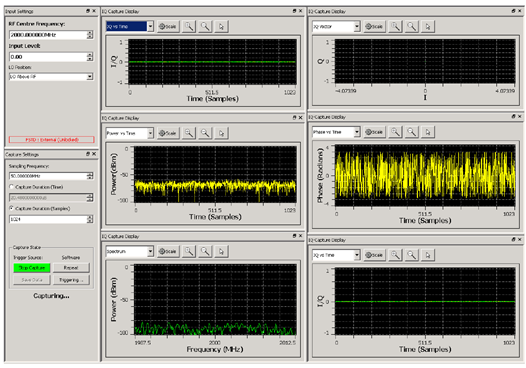
\includegraphics[scale=1.0]{ax518_soft}
	\caption{Программный модуль системы тестирования электронных устройств AX518~\cite{AX518}}
	\label{fig:lit_reiview:analogues:ax518_soft}
\end{figure}

\subsection{Аналитический обзор}
\label{sub:lit_review:analitics}
Технические средства(ТС) --  изделия, оборудование, аппаратура и их составные части, функционирующие на основании законов электротехники, радиотехники и электроники и содержащие электронные компоненты и схемы.

КМУ -- комплекс машин управления.
В состав комплекса машин управления огнем входят:
\begin{itemize}
	\item машина управления командира дивизиона~\cite{div_car}
	\item командно-штабная машина дивизиона
	\item машина управления командира батареи
	\item машина управления старшего офицера батареи
\end{itemize}

\begin{figure}[ht]
	\centering
	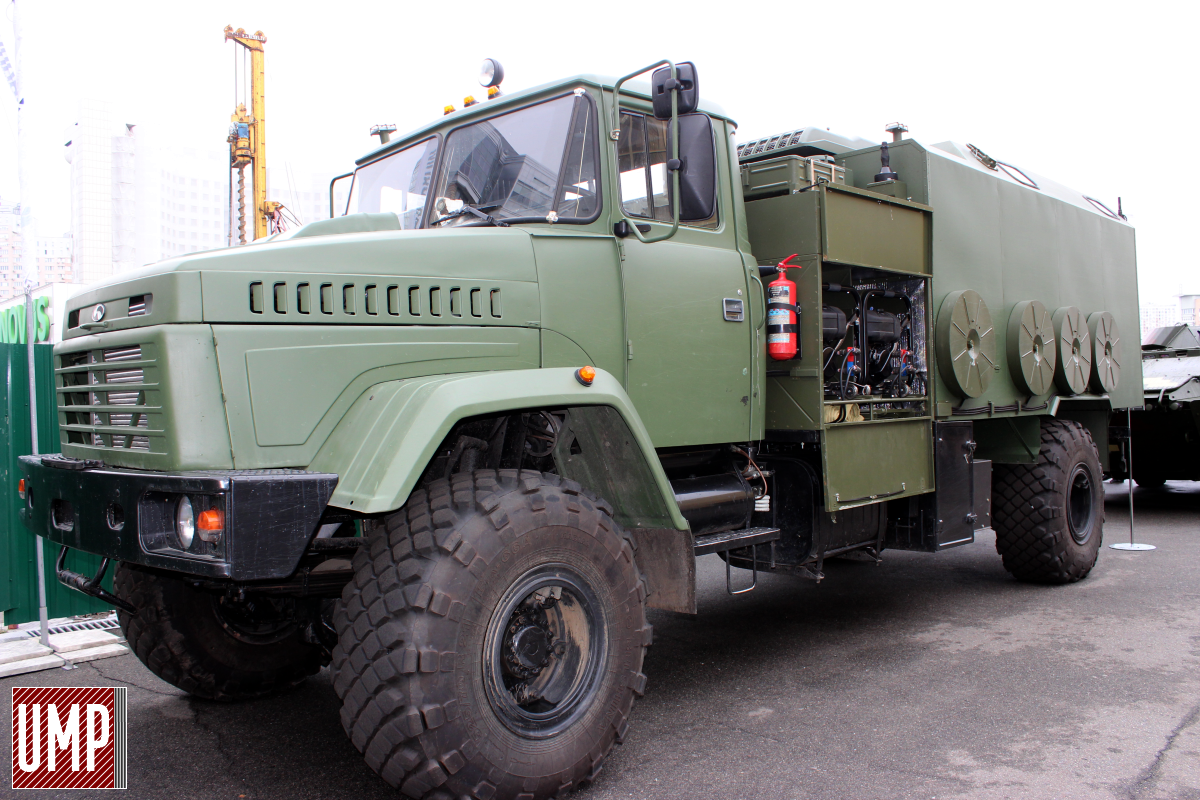
\includegraphics[scale=0.33]{div_com}
	\caption{Машина начальника штаба дивизиона на колесном шасси~\cite{div_car}}
	\label{fig:lit_reiview:analytics:div_com}
\end{figure}
В одном дивизионе имеется несколько машин разного уровня управления, содержащих в своем составе разные ТС.
Например, метеокомплект стоит только на нескольких машинах, радиостанции имеются в каждой машине, бесплатформенная
инерциальная навигационная система(БИНС) присутствует также на каждой машине, но имеют разные типы устройства, локальная
вычислительная сеть(ЛВС) присутствует в каждой машине.\break\break
Программное обеспечение написано для всех машин КМУ с возможностью выборки подключенных ТС.

Разработанное в ходе дипломного проектирования программное обеспечение предназначено для развертывания в подвижном
комплексе средств автоматизации управления~\cite{patent_2263960}.
Этот подвижный комплекс средств автоматизации управления, размещенный в подвижном объекте на шасси автомобиля повышенной
грузоподъемности, содержит несколько автоматизированных рабочих места(АРМ) должностных лиц, размещенных в кузове-фургоне
подвижного объекта, оборудованных средствами вычислительной техники и средствами передачи данных, радиорелейную станцию
с антеннами, коротковолновую (KB) радиостанцию, две ультракоротковолновые (УКВ) радиостанции, локальную вычислительную
сеть (ЛВС), специальный принтер.

\begin{figure}[ht]
	\centering
	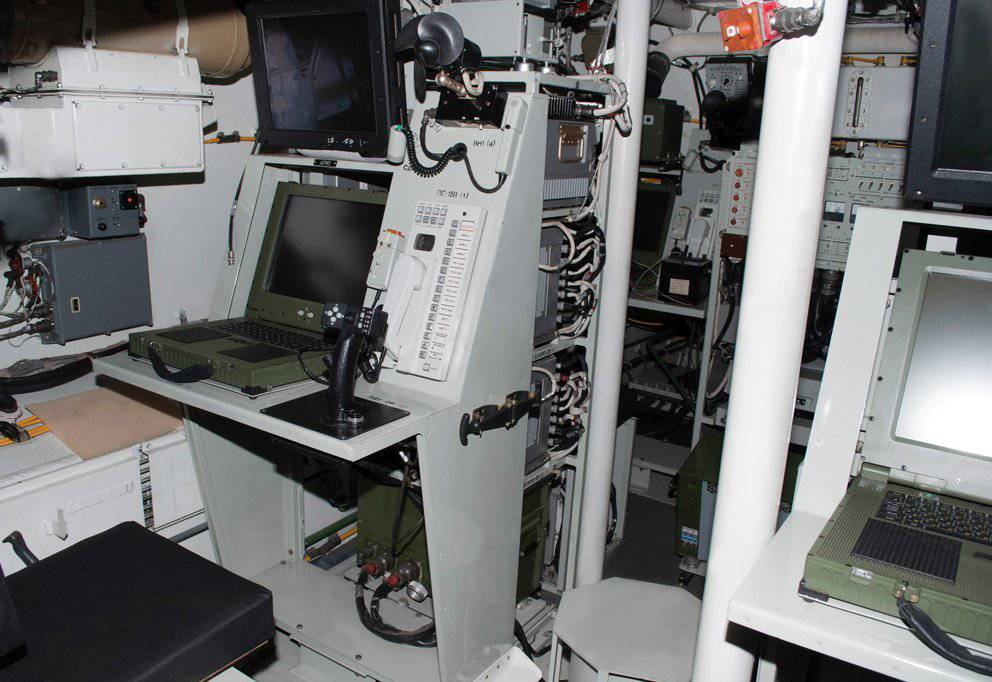
\includegraphics[scale=0.40]{arm}
	\caption{Автоматизированное рабочее место~\cite{patent_2263960}}
	\label{fig:lit_reiview:analytics:arm}
\end{figure}

Программа функционального контроля предназначена для осуществления автоматизации процессов проведения тестирования
технических\break средств.
Программа функционального контроля обеспечивает выполнение\break следующих функций:
\begin{enumerate}
\item тестирование средств автоматизации, локальной вычислительной\break сети(ЛВС), визуализацию информации о доступных в ЛВС автоматизированных рабочих местах(АРМ);
\item тестирование и настройку средств связи;
\item тестирование и настройку средств измерения.
\end{enumerate}

\subsection{Интегрированный навигационно-информационный комплекс}
\label{sub:lit_review:ins}

Интегрированный навигационно-информационный комплекс это комплексная бесплатформенная система ориентации и навигации,
построенная с использованием высокоточных акселерометров и волоконно-оптических гироскопов с замкнутым контуром,
построена на принципе комплексирования данных бесплатформенной инерциальной системы (БИНС) с одометром, приемником спутниковых навигационных сигналов (СНС)\break GPS/GLONASS и приемником барометрического давления.
ИНИК имеет модульную систему, которая позволяет получить различные варианты системы, наиболее полно удовлетворяющие потребности по точности измерений, удобству размещения на объекте.

Аппаратура позволяет  решать весь комплекс задач топопривязки, навигации и ориентирования средств ракетных войск и артиллерии в любое время в любых погодных условиях независимо от доступности сигналов СНС:
\begin{itemize}
	\item определение текущих координат объекта на стоянке (огневой позиции, районе сосредоточения), в ходе совершения марша
	\item определение углов ориентации подвижных объектов (азимутального угла продольной оси машины, углов крена и тангажа)
	\item автоматическое определения по сигналам спутниковых навигационных систем (далее СНС) GPS/GLONASS текущего единого и местного времени с использованием поправок на часовой пояс
	\item отображение на мониторе бортовой ЭВМ, индикаторных панелях текущих значений координат и высоты, а также скорости, угла продольной оси машины
	\item отображение на мониторе бортовой ЭВМ навигационной и топогеодезической информации на электронных картах местности собственного местоположения
\end{itemize}

Состав интегрированного навигационно-информационного комплекса:
\begin{itemize}
	\item блок спутниковый навигационный (БСН) с цифровым датчиком атмосферного давления
	\item цифровой одометрический датчик пути
	\item блок управления и обработки данных
	\item блок инерциальный навигационный измерительный на основе высокоточных акселерометров и волоконно-оптических гироскопов
\end{itemize}

Ниже приведен краткий обзор компонентов комплекса INS.

\subsubsection{Бортовая ЭВМ}
\label{sub:lit_review:ins:evm}
ПЭВМ серии БК402 служит для выполнения вычислительных функций в подвижных объектах на гусеничном и колесном ходу в закрытых кузовах
как на стоянке так и в движении. Возможно также использование ПЭВМ в стационарных условиях~\cite{bk402}.

Состав ПЭВМ:
\begin{itemize}
	\item машина вычислительная серии БК402;
	\item комплект периферийного оборудования, включающий в себя видеомониторы серии ВМЦ, клавиатуру, манипулятора графической информации (МГИ).
\end{itemize}.

ПЭВМ выполняет вычислительные функции, функции управления объектами, а также функции ввода-вывода, хранения, отображения и обработки информации.
ПЭВМ может  использоваться в  качестве:
\begin{itemize}
	\item центральной ЭВМ;
	\item автоматизированного рабочего места, при подключении видеомонитора, клавиатуры, манипулятора графической информации (МГИ).
\end{itemize}

Особенности и преимущества ПЭВМ:
\begin{itemize}
	\item наличие встроенного коммутатора на 4 порта, позволяющего применять данную модификацию для  построения локальных вычислительных сетей без применения внешнего коммутатора.
	\item наличие элементов крепления для установки их в подвижном объекте.
	\item наличие в корпусе амортизационной платформы и внутренних амортизаторов, обеспечивающих  выполнение требований к механическим воздействиям.
\end{itemize}

\begin{figure}[ht]
	\centering
	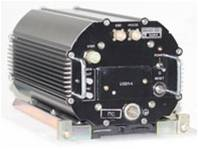
\includegraphics[scale=1.2]{bk402}
	\caption{Бортовая персональная электронная вычислительная машина серии БК402~\cite{bk402}}
	\label{fig:lit_reiview:ins:evm:bk402}
\end{figure}

\subsubsection{Бесплатформенная инерциальная навигационная система}
\label{sub:lit_review:ins:bins}
БИНС -- это бесплатформенная инерциальная навигационная система на волоконно-оптических гироскопах.
БИНС -- предназначена для определения параметров движения, угловой ориентации и параметров движения наземных
транспортных средств~\cite{bins}.

Навигационная система построена на базе кварцевых акселерометров и волоконно-оптических гироскопов. Точность применяемых чувствительных элементов позволяет БИНС-Тек работать как в режиме коррекции от спутниковой навигационной системы, так и в автономном инерциальном режиме с коррекцией от одометра.

БИНС не содержит металлических частей, подверженный усталостному напряжению (карданов подвес и т.п.) и не требует технического обслуживания в процессе эксплуатации.

Режимы определения навигационных параметров:
\begin{itemize}
	\item инерциальная навигационная система;
	\item спутниковая навигационная система.
\end{itemize}
\begin{figure}[ht]
	\centering
	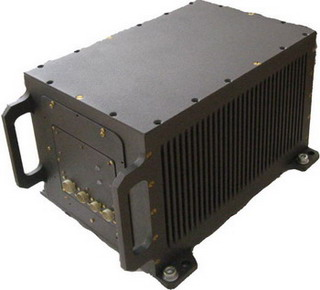
\includegraphics[scale=3.0]{bins}
	\caption{Бесплатформенная инерциальная навигационная система БИНС-Тек~\cite{bins}}
	\label{fig:lit_reiview:ins:bins}
\end{figure}

\subsection{Многофункциональная программно-определяемая радиостанция}
\label{sub:lit_review:radio}

Радиостанции предназначены для обеспечения передачи открытой и защищенной информации (речевых сообщений и данных) с
повышенной помехозащищенностью и скрытностью~\cite{prc9661}.
В каждой машине КМС установлено несколько радиостанций различных типов.

Применение радиостанций:
\begin{itemize}
	\item тактическое звено управления вооруженных сил
	\item использование в танках, БМП, БТР, автомобилях
	\item оснащение воинских подразделений наблюдения и разведки, должностных лиц уровней командования батальонами (дивизионами), ротами (батареями) и взводами
	\item оснащение командных пунктов вооруженных сил пунктов управления и узлов связи рот, батальонов и бригад
\end{itemize}

\begin{figure}[ht]
	\centering
	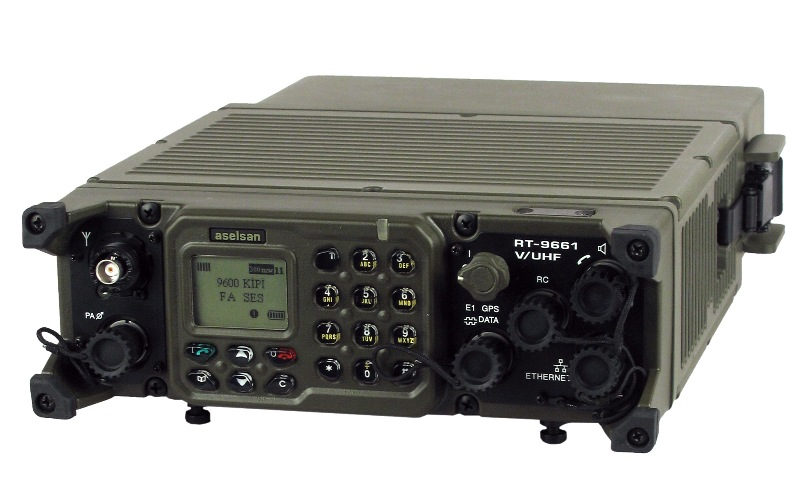
\includegraphics[scale=0.33]{radio_station}
	\caption{Радиостанция серии <<Р-181>> <<Рапсодия>>~\cite{prc9661}}
	\label{fig:lit_reiview:meteo:radio_station}
\end{figure}

\subsubsection{Блок спутниковый навигационный}
\label{sub:lit_review:ins:bsn}
Блок спутниковый навигационный (БСН) с цифровым датчиком атмосферного давления предназначен для приема сигналов ГЛОНАСС/GPS, включает защищенную антенну и малогабаритный приемник-измеритель.
\begin{figure}[ht]
	\centering
	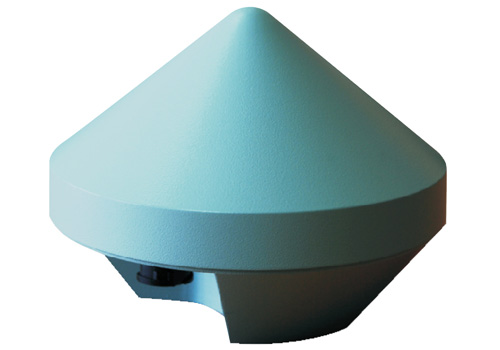
\includegraphics[scale=1.0]{bsn}
	\caption{Блок спутниковый навигационный~\cite{bsn}}
	\label{fig:lit_reiview:ins:bsn}
\end{figure}

\subsubsection{Блок управления и обработки сигналов}
\label{sub:lit_review:ins:bos}
Блок управления и обработки сигналов (БОС) предназначен для обработки сигналов принимаемых от бесплатформенной
навигационной системы, блока спутникового навигационного, цифрового датчика пути, их
формирования и передачи на бортовую ЭВМ.

\subsection{Автоматическая метеостанция}
\label{sub:lit_review:meteo}

Автоматическая метеостанция(АМС) это комплексный универсальный метеорологический модуль - компактное и легкое
устройство, оснащенное набором датчиков, необходимых для измерения основных метеорологических величин ~\cite{wxt530}:
\begin{itemize}
	\item направления и скорости ветра
	\item атмосферного давления
	\item температуры и относительной влажности
\end{itemize}

АМС с успехом применяется в ракетных войсках и артиллерии для определения метеорологических условий стрельбы, расчет суммарных поправок на отклонение условий стрельбы.
Модуль легко устанавливается на штатной штанге командно-штабной машине дивизиона с помощью одного винта.
Поскольку модуль не имеет движущихся частей, он надежен в эксплуатации и практически не требует обслуживания.
Используемые материалы обладают высокой устойчивостью к различным загрязнения и суровым погодным условиям.
Модуль соединяется с приемным устройством двунаправленной линией передачи.

\begin{figure}[ht]
	\centering
	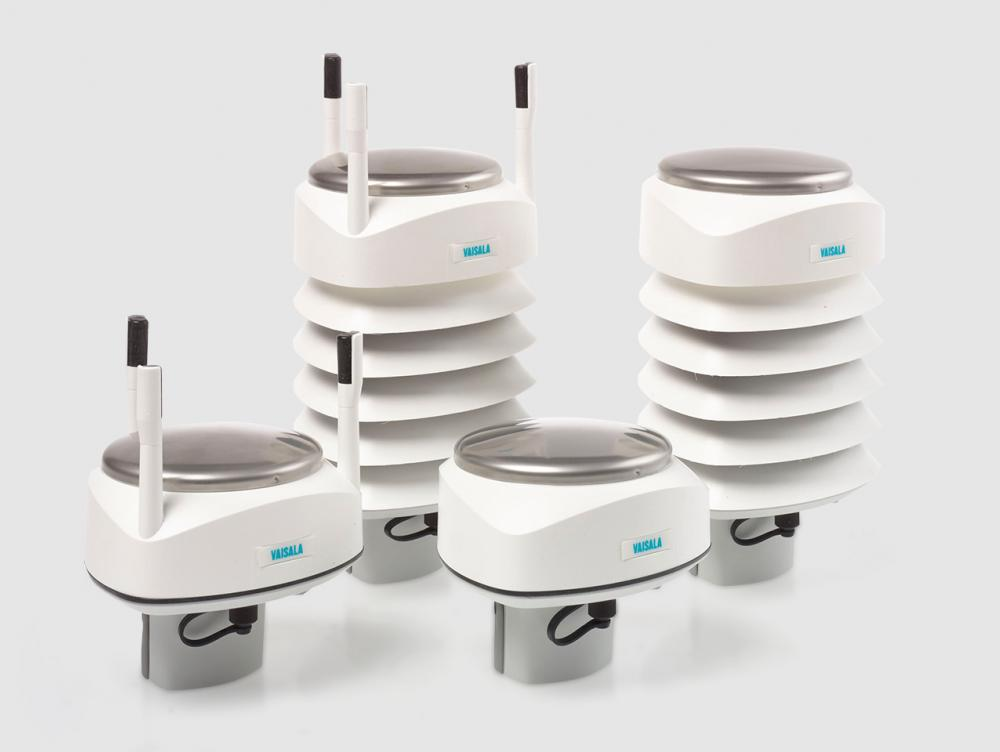
\includegraphics[scale=0.3]{meteo_station}
	\caption{Автоматическая метеостанция WXT530~\cite{wxt530}}
	\label{fig:lit_reiview:meteo:meteo_station}
\end{figure}

\subsection{Специальный принтер}
\label{sub:lit_review:spec_printer}
Специальный принтер предназначен для эксплуатации в составе мобильных вычислительных комплексов.
Может эксплуатироваться в процессе движения транспортных средств ~\cite{mp2200}.

Наиболее удобным для эксплуатации в машине КМУ является термопринтер. Термопринтеры гораздо более устойчивы к вибрациям и ударам, чем лазерные, матричные и струйные принтеры.

Корпус выполнен из металла, что обеспечивает стойкость к внешним механическим воздействиям.
Разъемы питания и интерфейсов (USB/LPT)\break принтера –высоконадежные «военные» байонетные металлические с металлической защитной заглушкой.
Интерфейс – высокоскоростной параллельный ECP/EPP и/или USB.

\begin{figure}[ht]
	\centering
	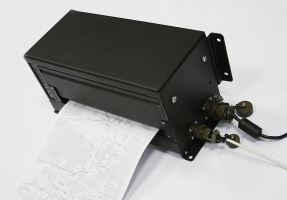
\includegraphics[scale=1.0]{printer}
	\caption{Специальный принтер МП2200~\cite{mp2200}}
	\label{fig:lit_reiview:spec_printer:printer}
\end{figure}

\subsection{Прибор-дальномер «Капонир»}
\label{sub:lit_review:kaponir}
Переносной телевизионно-тепловизионный наблюдательный прибор-дальномер «Капонир» предназначен для круглосуточного
ведения разведки противника и местности, определения координат своего местоположения, измерения дальности до объекта
(цели) и автоматического определения координат объекта (цели)~\cite{kaponir}.

Прибор имеет оптический, телевизионный и тепловизионный каналы наблюдения. Телевизионный и тепловизионный каналы позволяют
вести наблюдение днем и ночью. Прибор  крепится на треноге, а также  позволяет ведение наблюдения с руки.

Прибор оснащен:
\begin{itemize}
	\item приемным телевизионным каналом на фотоприемной матрице;
	\item приемным тепловизионным каналом на неохлаждаемой микроболометрической матрице;
	\item каналом лазерного дальномера;
	\item модулем электронного компаса - инклинометра;
	\item системой позиционирования GPS, ГЛОНАСС;
	\item системой расчета и определения координат объекта (цели).
	\item окуляром с OLED-микродисплеем (дисплеем на основе плоскостных органических светодиодов).
\end{itemize}

\begin{figure}[ht]
	\centering
	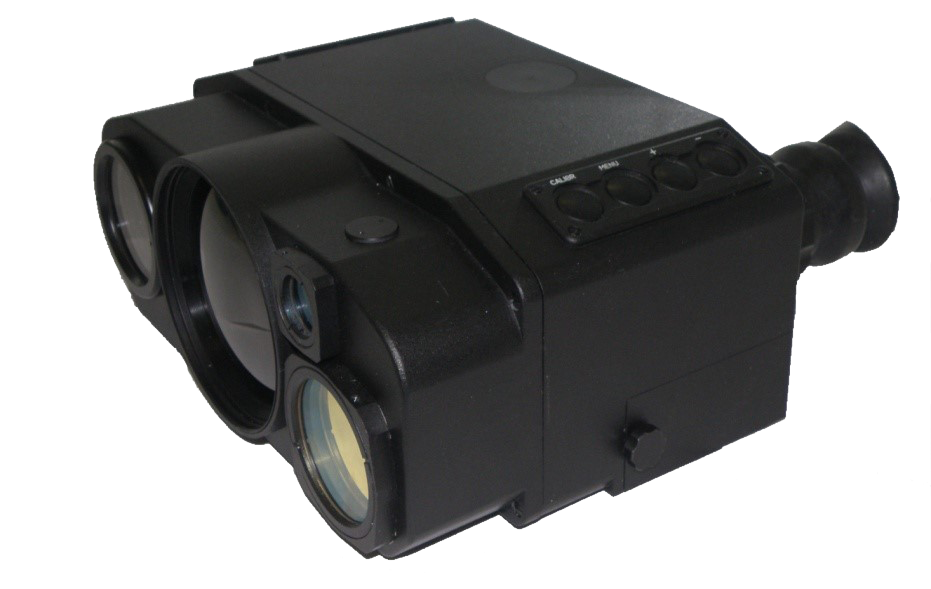
\includegraphics[scale=1.0]{kaponir_img}
	\caption{Прибор-дальномер <<Капонир>>~\cite{kaponir}}
	\label{fig:lit_reiview:kaponir:kaponir_img}
\end{figure}

\subsection{Лазерный целеуказатель-дальномер}
\label{sub:lit_review:lcd}
Лазерный целеуказатель-дальномер 1Д22 предназначен для разведки целей и обслуживания стрельбы наземной и корабельной
артиллерии обычными и высокоточными артиллерийскими боеприпасами с полуактивной лазерной системой наведения, а
также для обеспечения применения высокоточных боеприпасов при подсветке лазерным излучением неподвижных и движущихся объектов
вооружения и военной техники, инженерных сооружений, для корректировки артиллерийского огня с выносных наземных наблюдательных
пунктов или из машин управления огнем~\cite{lcd}.

Прибор ЛЦД обеспечивает: 
\begin{itemize}
	\item ведение разведки противника и местности;
	\item измерение горизонтальных и вертикальных углов, (имеется селекция целей и система стробирования);
	\item измерение дальности до целей (объектов), разрывов снарядов (мин);
	\item осуществление целеуказания (лазерный подсвет цели) при наведении управляемых артиллерийских боеприпасов.
\end{itemize}

\begin{figure}[ht]
	\centering
	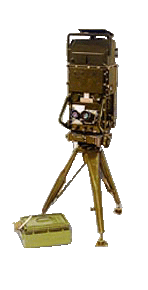
\includegraphics[scale=1.0]{lcd_img}
	\caption{Лазерный целеуказатель-дальномер 1Д22~\cite{lcd}}
	\label{fig:lit_reiview:lcd:lcd_img}
\end{figure}
